\section{Methods and Implementation}\label{methods and implementation}

This section presents different processing techniques with the aim of solving the task at hand. SEALAB's current solutions is explained and discussed. The new implementation is explained step by step followed by images showing the process and the results.


\subsection{Previous implementation done by SEALAB}

Before the start of this project, setup of all needed hardware and software was already accomplished. Also, some implementation had already been made and some enhancement on the depthmap image was already tried out.

The Raytrix camera needs to be attached to a computer and the computer along with the raytrix software is used when taking images. One difficulty is that the depth information is stored in its own .ray format, and since this format is not known to other processing tools it needs to be converted. SEALAB already has a program using C++ and OpenCV that converts this .ray file to a .png image holding the depthmap. 

Already in place is also the actual algorithm calculating the volume of an object. This algorithm currently uses the depth information directly from the raytrix software and does not take a .png depthmap image. For the results developed in this report the volume measurement algorithm needs to receive the right depth information represented by the colors in the depthmap. This is most likely done by receiving data both from the .ray file along with the enhanced depthmap image.

SEALAB has already tried using interpolation algorithms for filling out the fish. The problem with this algorithm is that its runtime is very slow, and the results are not sufficient. The colors along the fish is very uneven. 


{\color{red}
Write about what they have already tried out. 
they have tried interpolation filling out the fish. Show picture of the green fish. 
This did work, but the interpolation algorithm take forever to run and you can see the colors that represent the depth of the fish is not that even.

What is also now done is get the p-data directly from the Raytrix software, then make a depthmap from the p-data and use the p-data in the volume algorithm. What I want to do is get the depthmap directly from the Raytrix, do some work on it, extract the p-data based on color, then send the data to through the volume algorithm. 
}

%%%%%%%%%%%%%%%%%%%%%%%%%%%%%%%%%%%%%%%%%%%%%%%%%%%%%%%%%%%%%%%%%%%%%%


\subsection{Depthmap enhancement} \label{section:depthmap}

The approach used to better the depthmap image is mostly based on color filtering followed by morphological closing together with object detection. 
Color filtering is first used to remove detected particles. All data, based on its color, too close to the camera or too far behind the object is removed. This is an easy way of filtering out irrelevant data. Morphological closing is a very good operation for leveling out the color and fill the holes, and it is therefore used several times in a row on the color filtered image. The only problem is that the object will lose its original shape when used many iterations in a row. To solve this problem, an object detection algorithm was run on the color filtered image. This algorithm finds the largest contour in the image and returns a mask of the contour. This mask is put on top of the morphologically closed image and makes the result.

The steps of the algorithm follows below, and the complete code can be found in section \ref{code}.

\begin{enumerate}
    \item \textbf{Filter out unwanted colors:}
    Color-filtering was done by looping through each pixel in the image and setting it to black if its blue-value was too high, green-value too low or red-value too low. This removed all particles detected by the Raytrix that was too close or to far behind. 
    
    \item \textbf{Remove small particles:}
    Removal of small particles was done by morphological opening. Too much closing would remove much of the fish, so here there is a fine line depending on how much depth data there is on the object.
    
    \item \textbf{Find largest contour:} 
    Finding the largest contour followed these steps: 
    \begin{enumerate}[label*=\arabic*.]
        \item Convert to grayscale and normalize
        \item Sobel edge detector and thresholding
        \item Dilate
        \item Floodfill
        \item Erode
        \item Find largest contour
    \end{enumerate}
    This algorithm is found on GitHub \cite{website:largest_contour_code_github}, but has been modified. For further explanation, see \cite{website:largest_contour_code_explanation}.
    The resulting images for each step of the algorithm is shown in figure \ref{fig:find_largest_contour}.
    
    \item \textbf{Morphological closing on color-filtered image:}
    To fill out the holes in the fish in an even way, morphological closing was used. This also levels out the depth data on the surface of the object.
    
    \item \textbf{Mask the morphological closed image with the largest contour:}
    Because the morphological closing operations would somewhere expand the object, the largest contour was used as a mask to gain the final result. 
\end{enumerate}

Figure \ref{fig:algorithm} shows the result after each step of the algorithm.

This approach was tested on different depthmap images, and gave very good results on many of them. It was also tested to find the largest contour from the totalfocus image instead of the depthmap, but the depthmap returned a more accurate contour. Figure \ref{fig:algorithm_test} shows the result of the algorithm from four different depthmaps of the same fish.
The result is good compared to the original depthmap, but the depthmap computed from the Raytrix software could be improved. This is most likely done by different lightning, or by giving the background a different color.
It was also tested when noise was added to the depthmap. This test and its results is explained in section \ref{section:noise}.

During the period of testing, the test facility in the wetlab was painted black. This point of this was to imitate open sea and try to point the light during image shooting directly towards the fish. It turned out that the lightning was too strong, and the fishes reflection too high to give any good results when pointing the light directly towards the fish. When focusing the light so that the depthmap was at its best, the previously experienced problems (from the white facility) with poor depth detection on the fishes belly, now just moved to bad detections on the fish's back.
This was therefore not as successful as hoped, but with different light conditions and various brightness the results can most likely improve.


\begin{figure}[H]
    \begin{subfigure}{0.48\textwidth}
        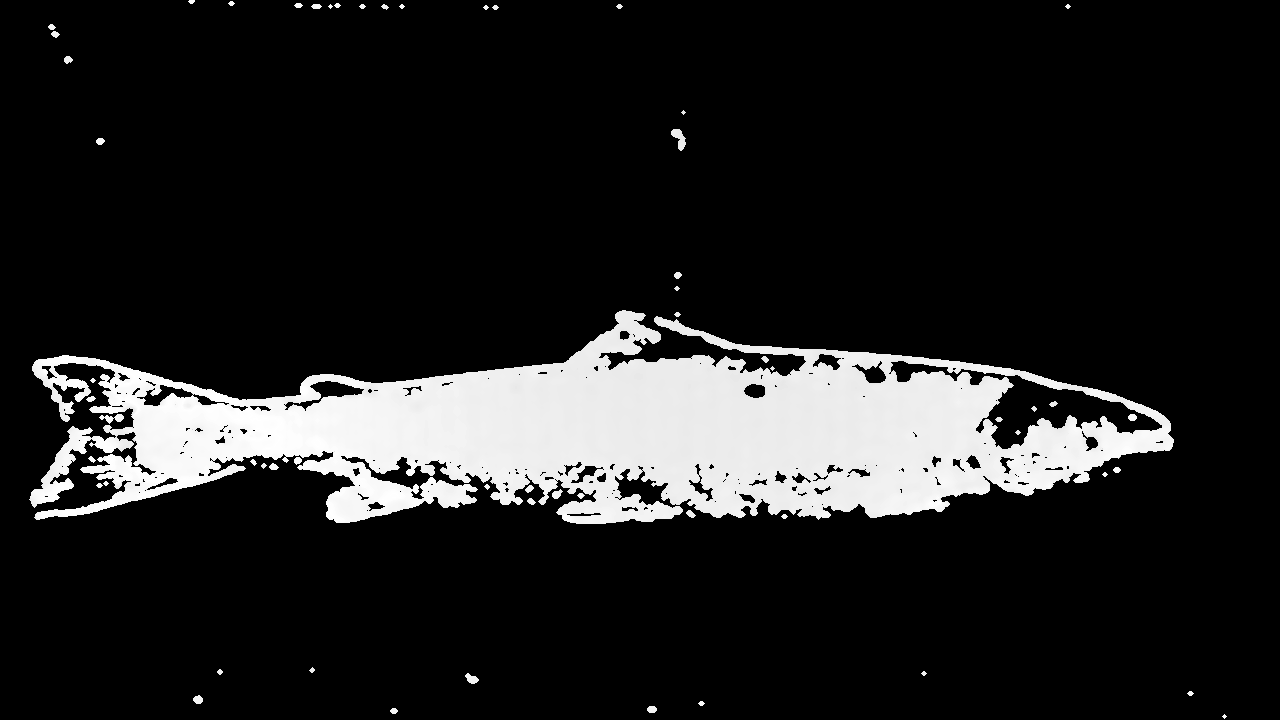
\includegraphics[width=\linewidth]{images/implementation/4_1_grayscale}
        \caption{Converted to grayscale} 
        \label{fig:grayscale}
    \end{subfigure}\hspace*{\fill}
    \begin{subfigure}{0.48\textwidth}
        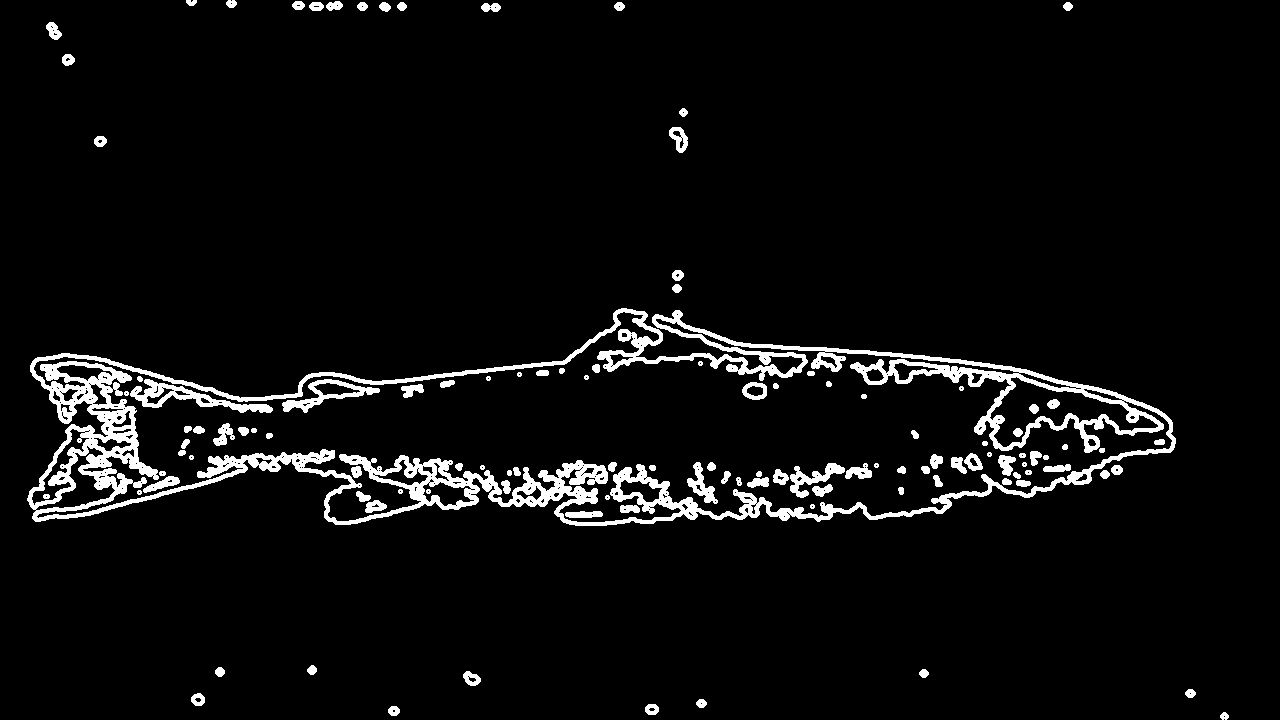
\includegraphics[width=\linewidth]{images/implementation/4_2_edge_detector}
        \caption{Edge detection} 
        \label{fig:edge_detection}
    \end{subfigure}
    
    \medskip
    \begin{subfigure}{0.48\textwidth}
        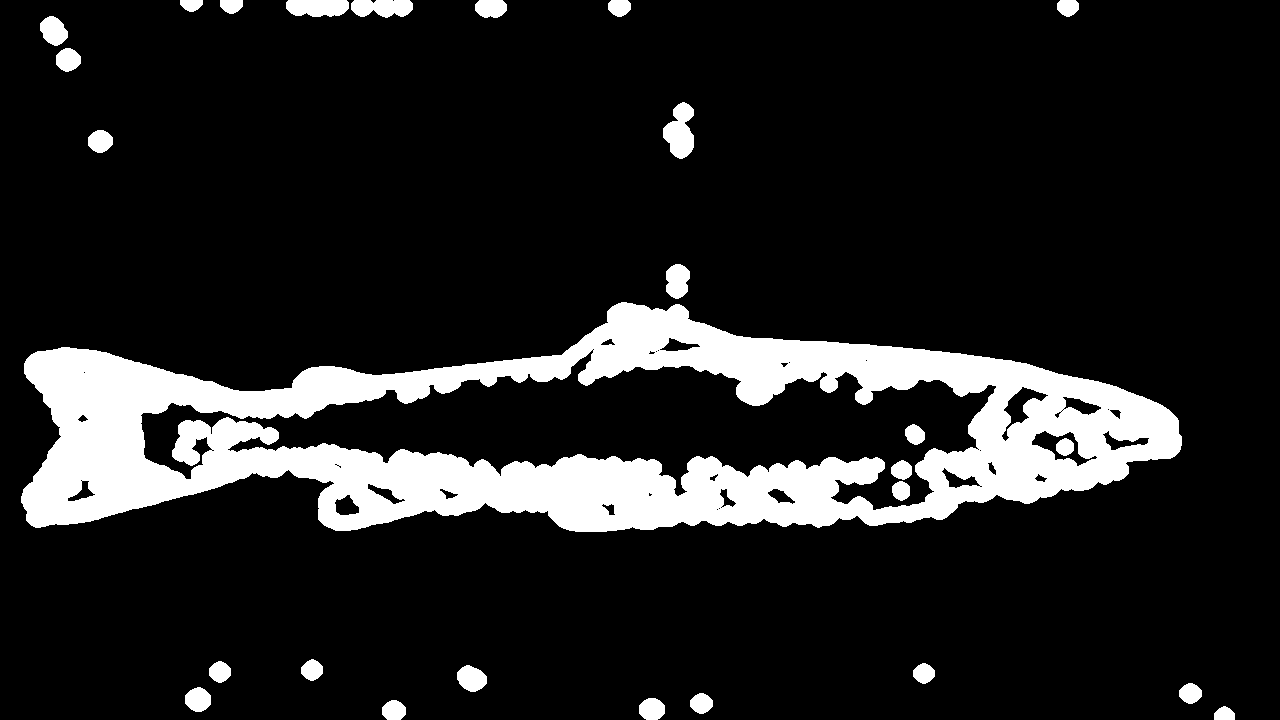
\includegraphics[width=\linewidth]{images/implementation/4_3_dilate}
        \caption{Dilate} 
        \label{fig:dilate_contour}
    \end{subfigure}\hspace*{\fill}
    \begin{subfigure}{0.48\textwidth}
        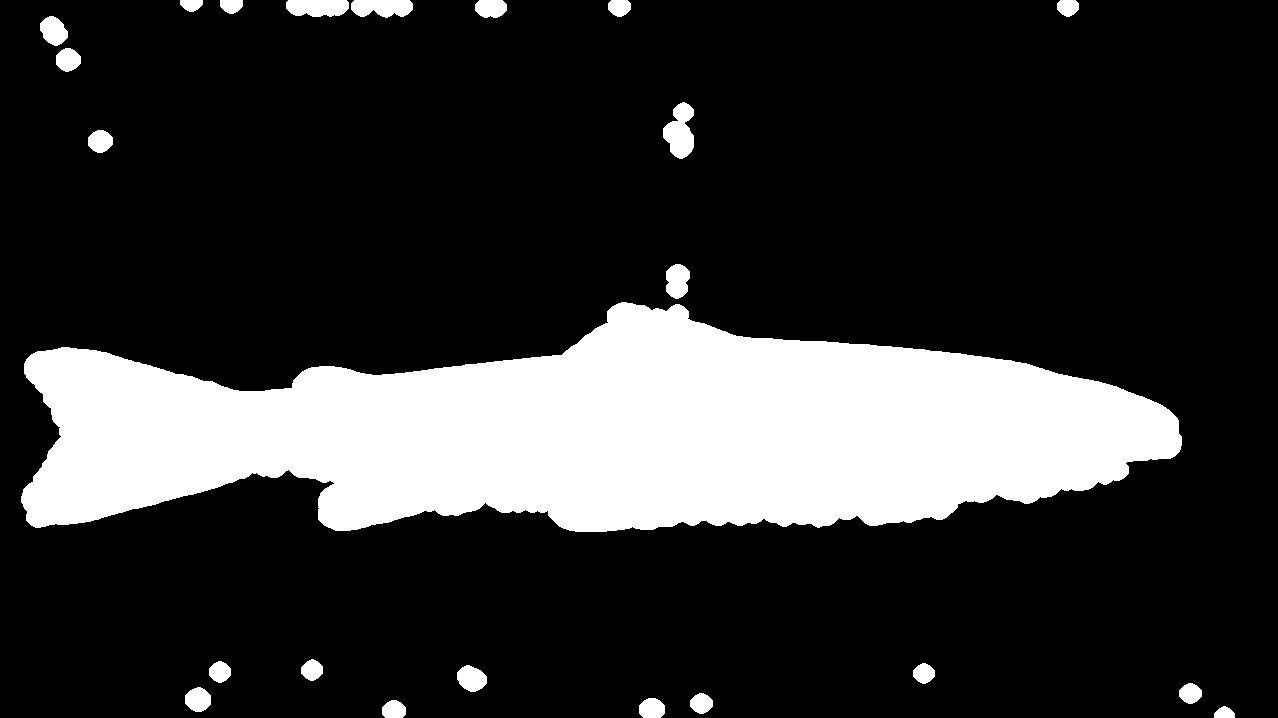
\includegraphics[width=\linewidth]{images/implementation/4_4_floodfill}
        \caption{Floodfill} 
        \label{fig:floodfill}
    \end{subfigure}
    
    \medskip
    \begin{subfigure}{0.48\textwidth}
        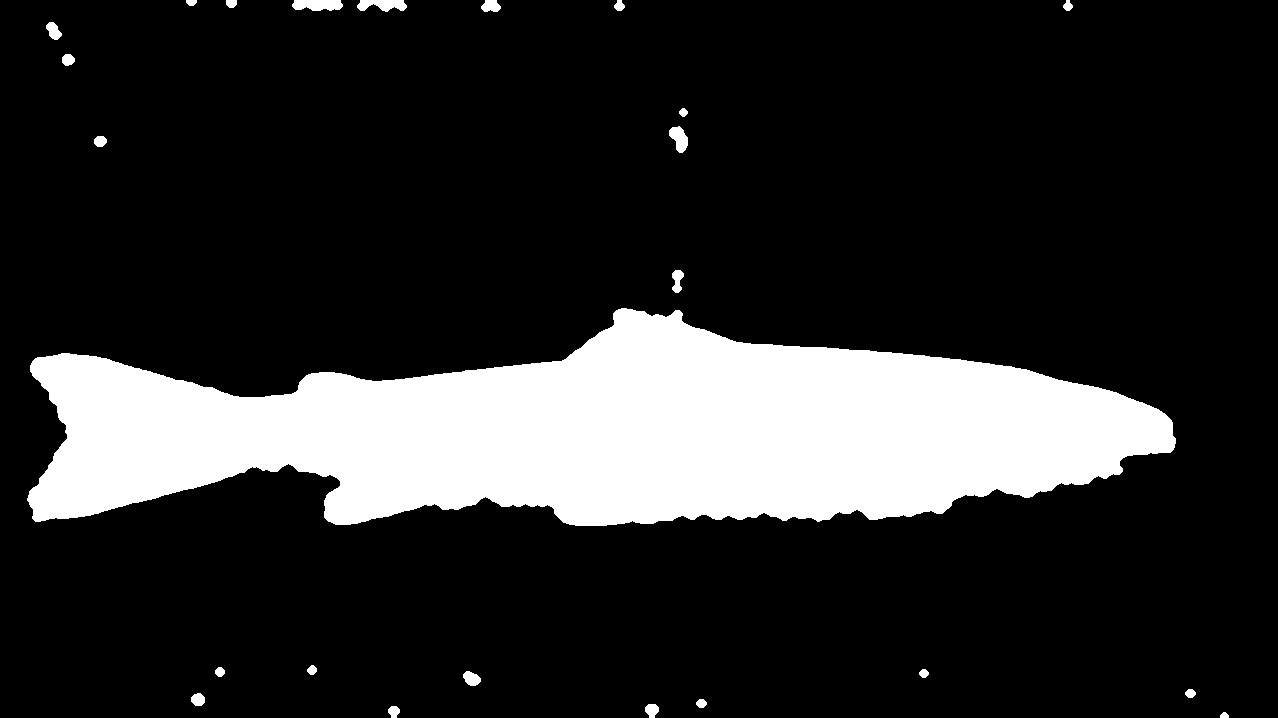
\includegraphics[width=\linewidth]{images/implementation/4_5_erode}
        \caption{Erode} 
        \label{fig:erode_contour}
    \end{subfigure}\hspace*{\fill}
    \begin{subfigure}{0.48\textwidth}
        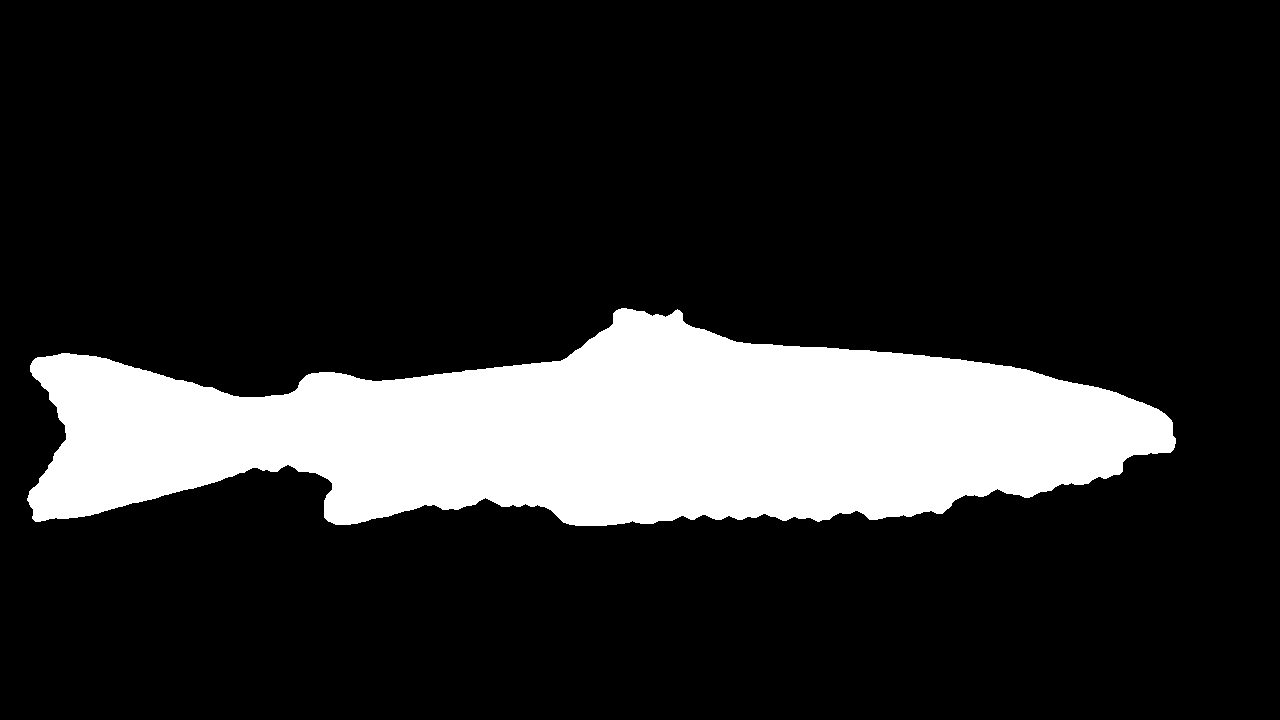
\includegraphics[width=\linewidth]{images/implementation/4_largest_contour}
        \caption{Largest contour} 
        \label{fig:largest_contour_2}
    \end{subfigure}
    \caption{Finding the largest contour} 
    \label{fig:find_largest_contour}
\end{figure}


\begin{figure}[H]
    \begin{subfigure}{0.48\textwidth}
        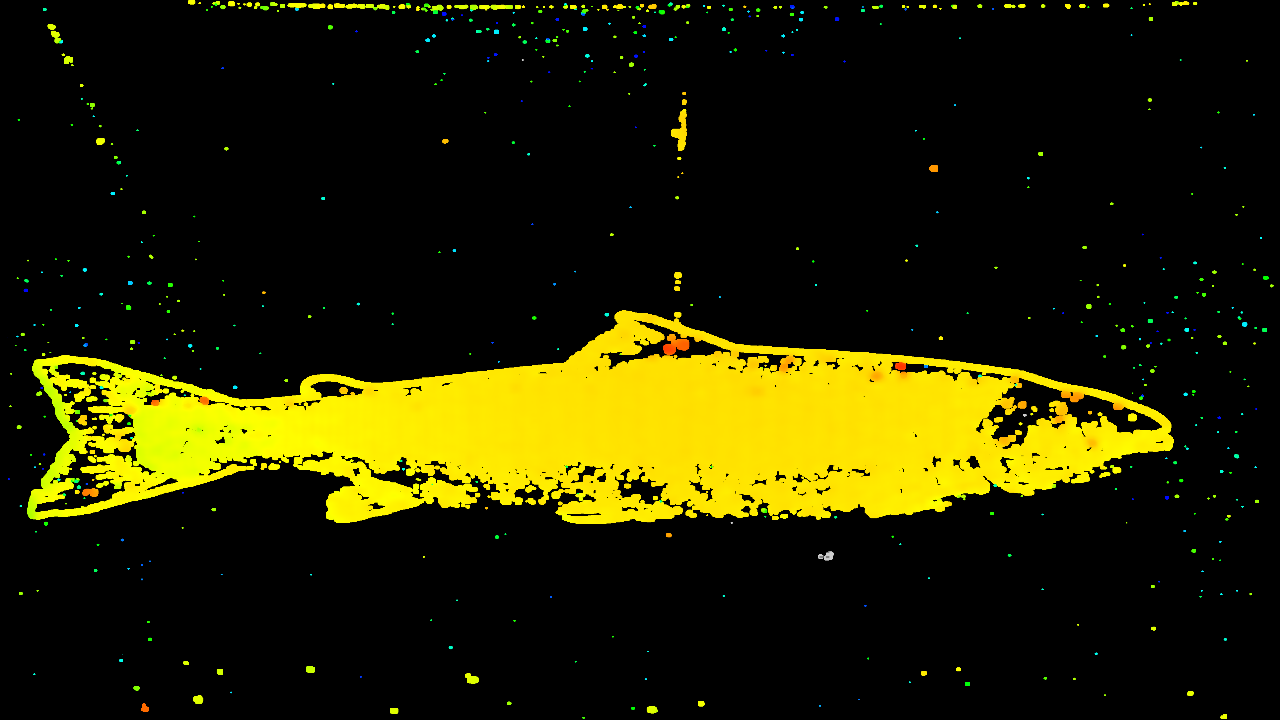
\includegraphics[width=\linewidth]{images/implementation/1_original}
        \caption{Original depthmap image} 
        \label{fig:original_depthmap}
    \end{subfigure}\hspace*{\fill}
    \begin{subfigure}{0.48\textwidth}
        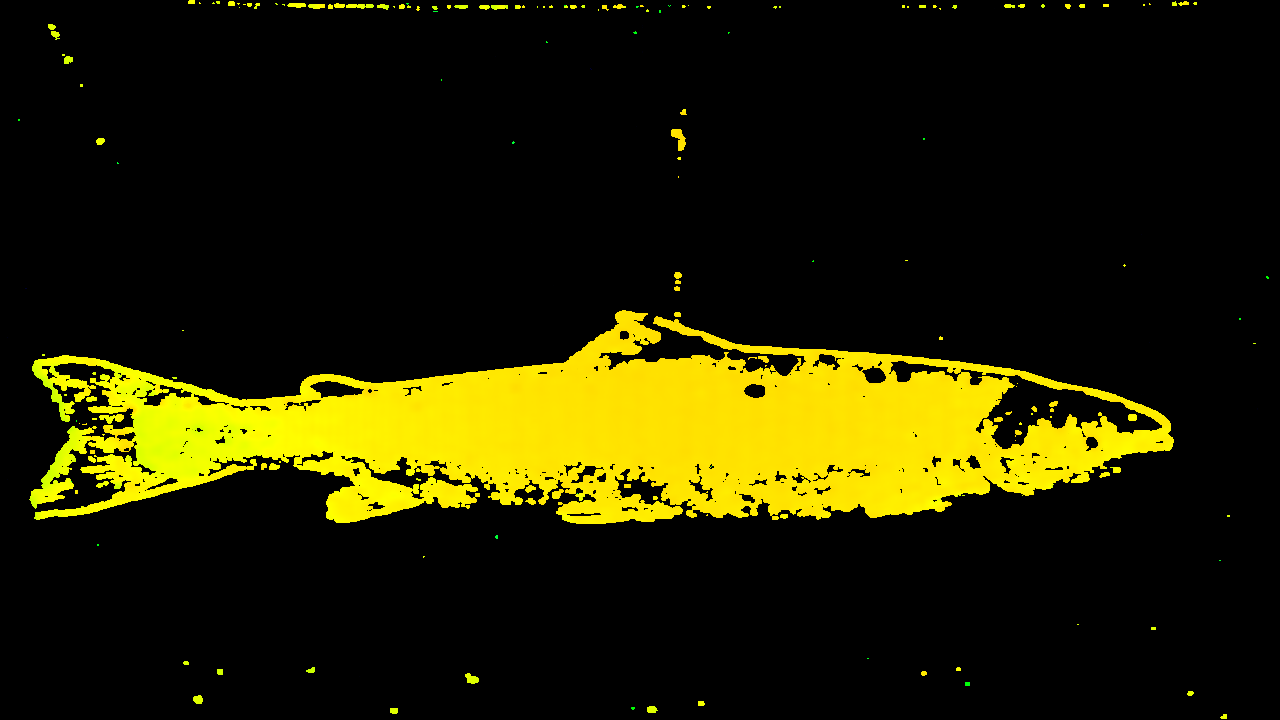
\includegraphics[width=\linewidth]{images/implementation/2_color_filtering}
        \caption{Color-filtered image} 
        \label{fig:color_filtering}
    \end{subfigure}
    
    \medskip
    \begin{subfigure}{0.48\textwidth}
        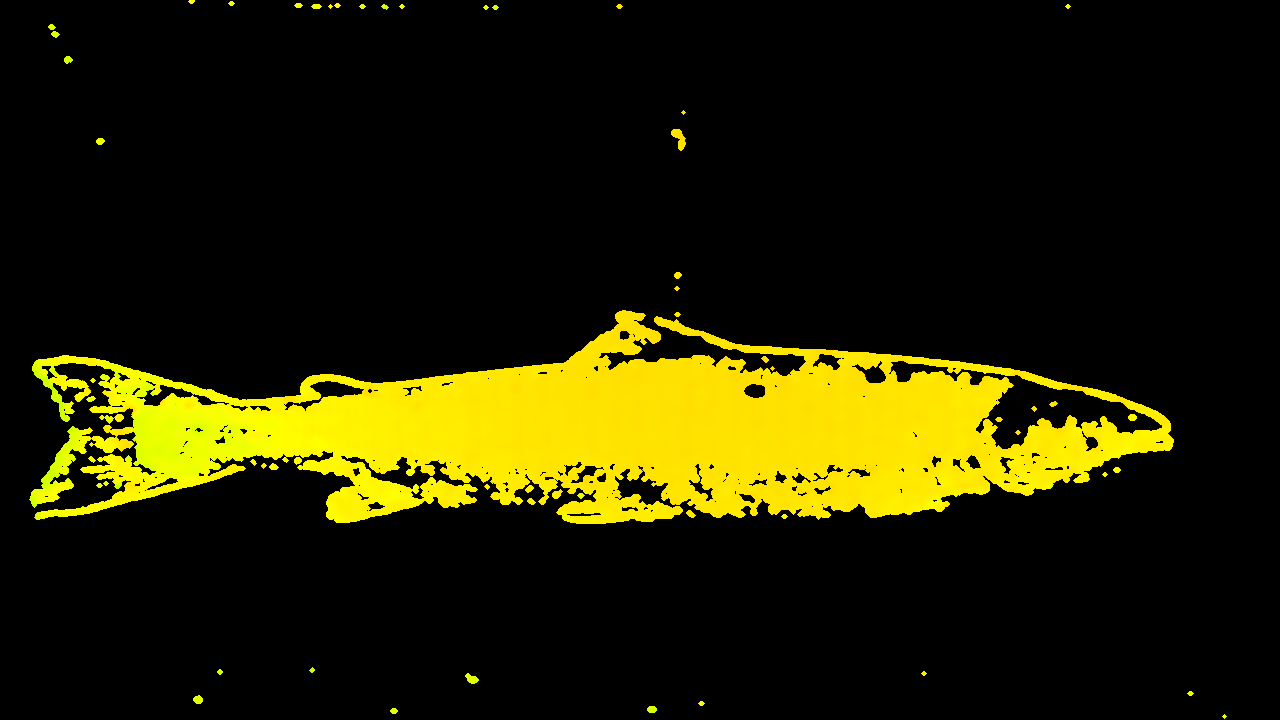
\includegraphics[width=\linewidth]{images/implementation/3_remove_particles}
        \caption{Removal of small particles} 
        \label{fig:remove_particles}
    \end{subfigure}\hspace*{\fill}
    \begin{subfigure}{0.48\textwidth}
        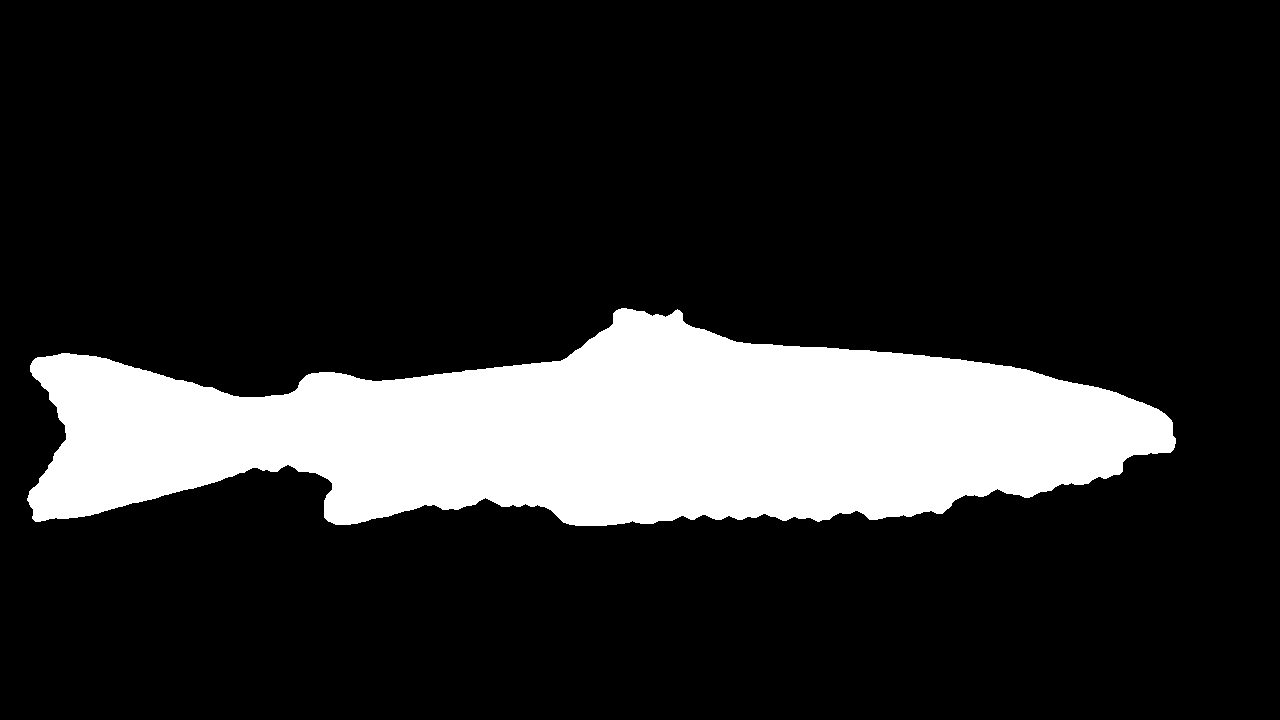
\includegraphics[width=\linewidth]{images/implementation/4_largest_contour}
        \caption{Largest contour} 
        \label{fig:largest_contour}
    \end{subfigure}
    
    \medskip
    \begin{subfigure}{0.48\textwidth}
        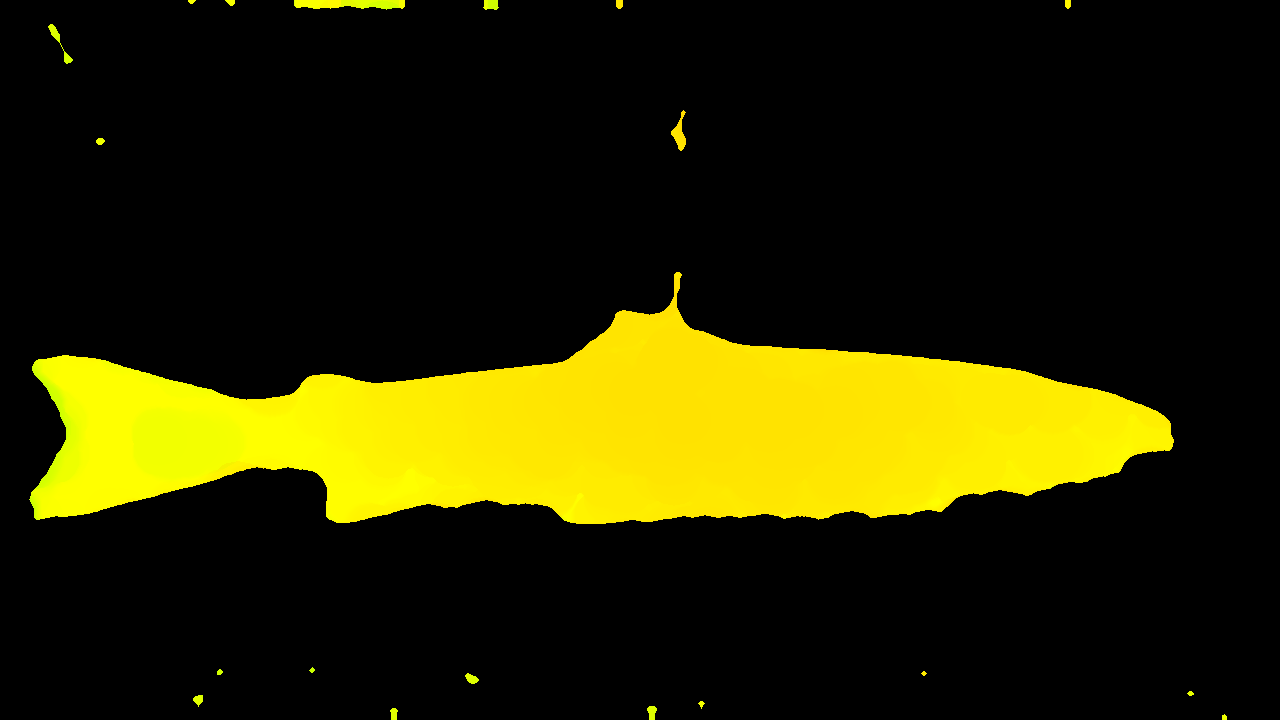
\includegraphics[width=\linewidth]{images/implementation/5_closing_on_color_filtered_image}
        \caption{Morphological closing} 
        \label{fig:morphological_closing}
    \end{subfigure}\hspace*{\fill}
    \begin{subfigure}{0.48\textwidth}
        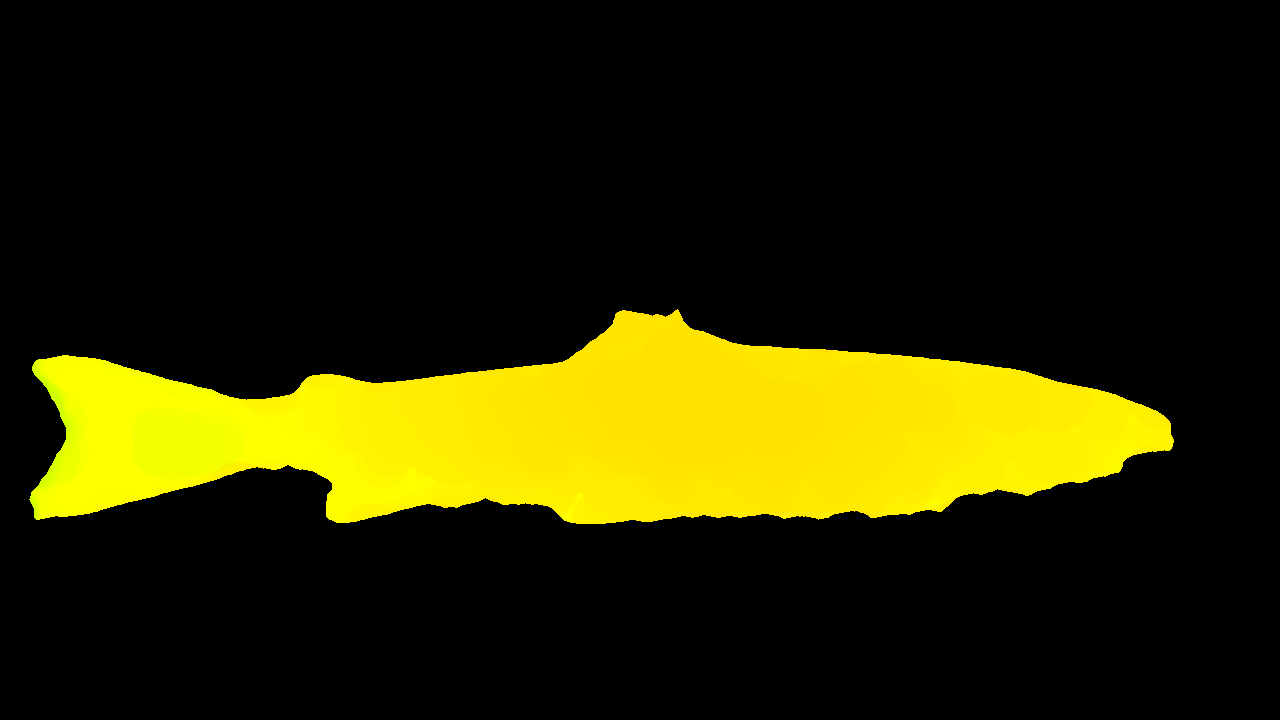
\includegraphics[width=\linewidth]{images/implementation/6_masked_source}
        \caption{Masked image} 
        \label{fig:masked_source}
    \end{subfigure}
    \caption{Morphological closing and masking with largest contour} 
    \label{fig:algorithm}
\end{figure}


\begin{figure}[H]
    \begin{subfigure}{0.48\textwidth}
        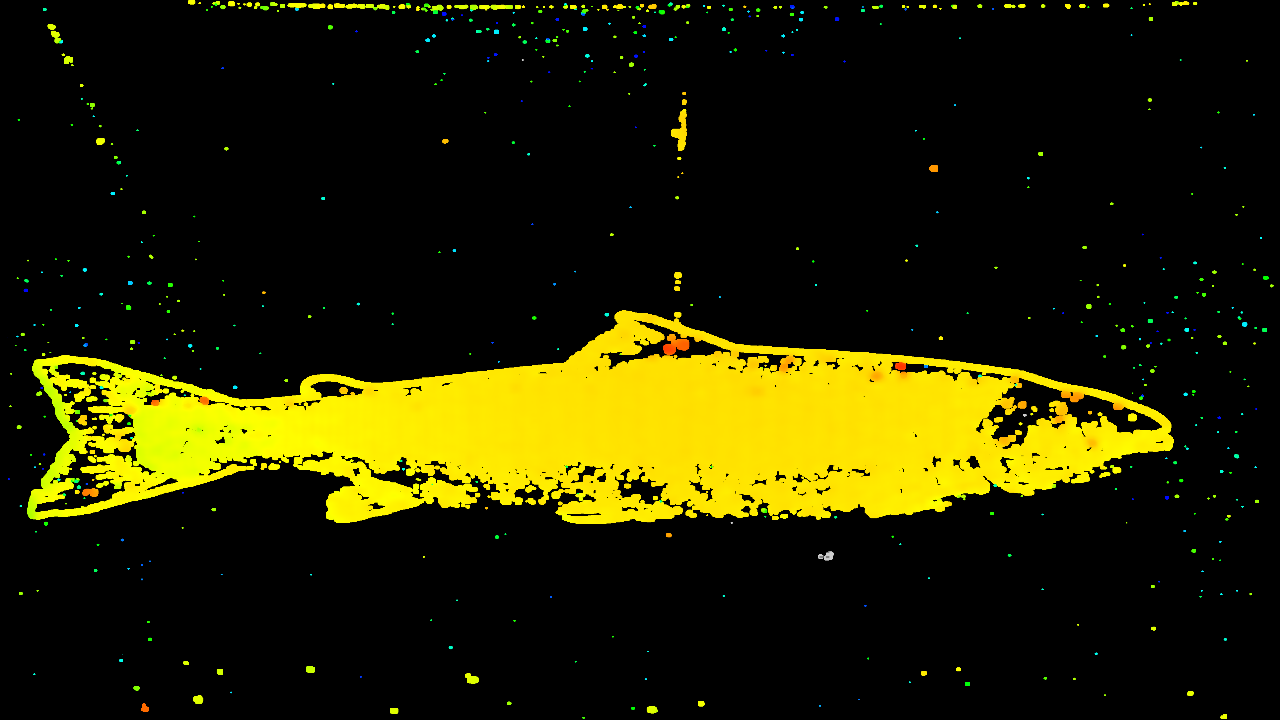
\includegraphics[width=\linewidth]{images/implementation/algorithm_test/original_63}
        \caption{Original depthmap image} 
        \label{fig:original_depthmap_63}
    \end{subfigure}\hspace*{\fill}
    \begin{subfigure}{0.48\textwidth}
        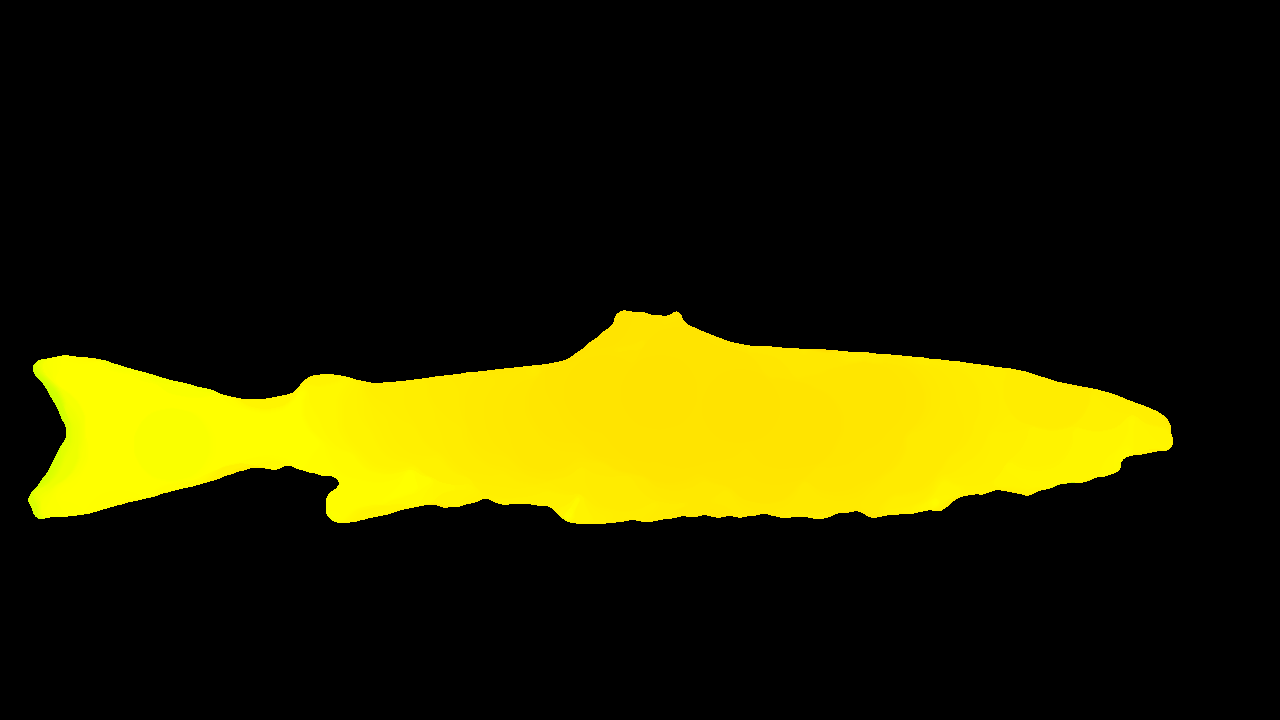
\includegraphics[width=\linewidth]{images/implementation/algorithm_test/median_filter_63}
        \caption{Result} 
        \label{fig:result_63}
    \end{subfigure}
    
    \medskip
    \begin{subfigure}{0.48\textwidth}
        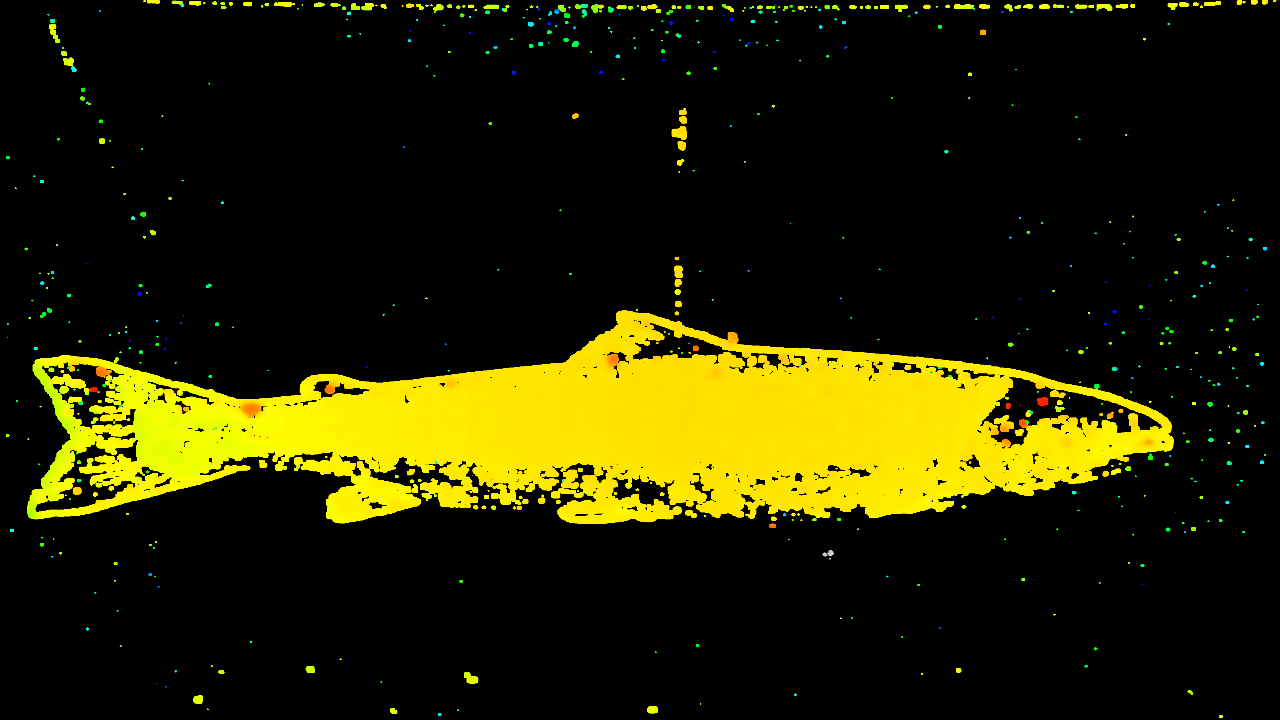
\includegraphics[width=\linewidth]{images/implementation/algorithm_test/original_73}
        \caption{Original depthmap image} 
        \label{fig:original_depthmap_73}
    \end{subfigure}\hspace*{\fill}
    \begin{subfigure}{0.48\textwidth}
        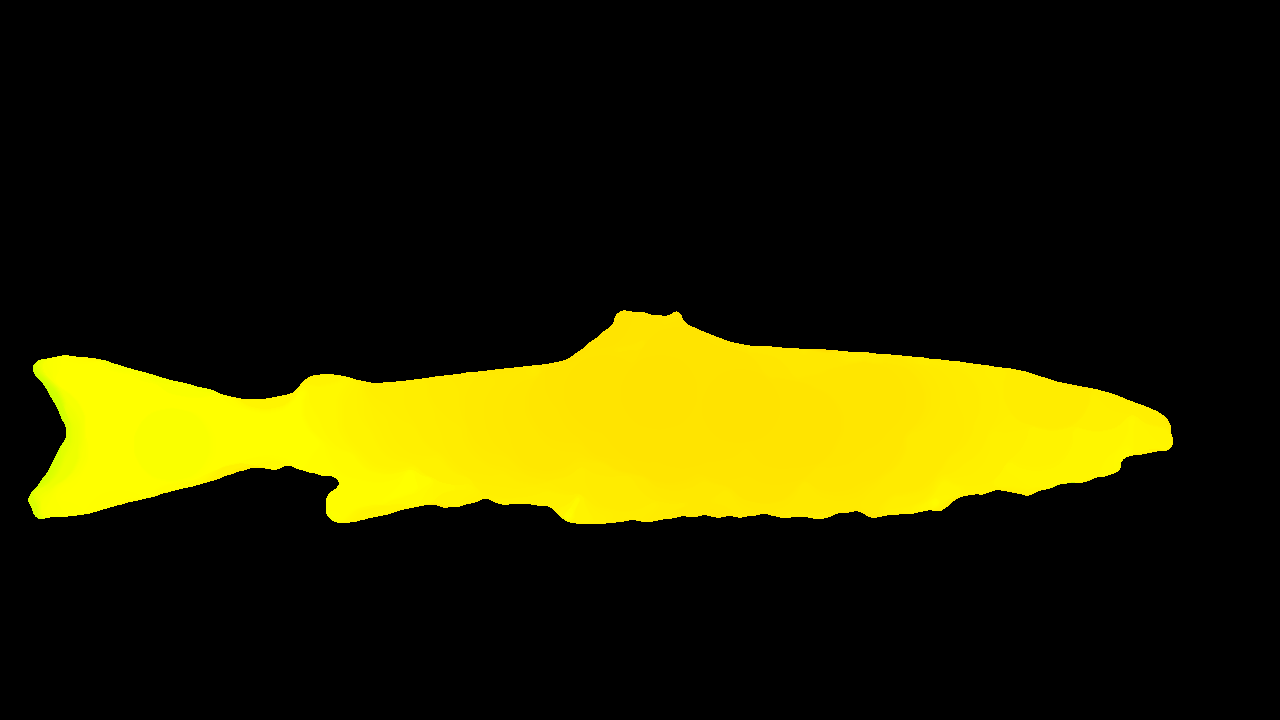
\includegraphics[width=\linewidth]{images/implementation/algorithm_test/median_filter_63}
        \caption{Result} 
        \label{fig:result_73}
    \end{subfigure}
    
    \medskip
    \begin{subfigure}{0.48\textwidth}
        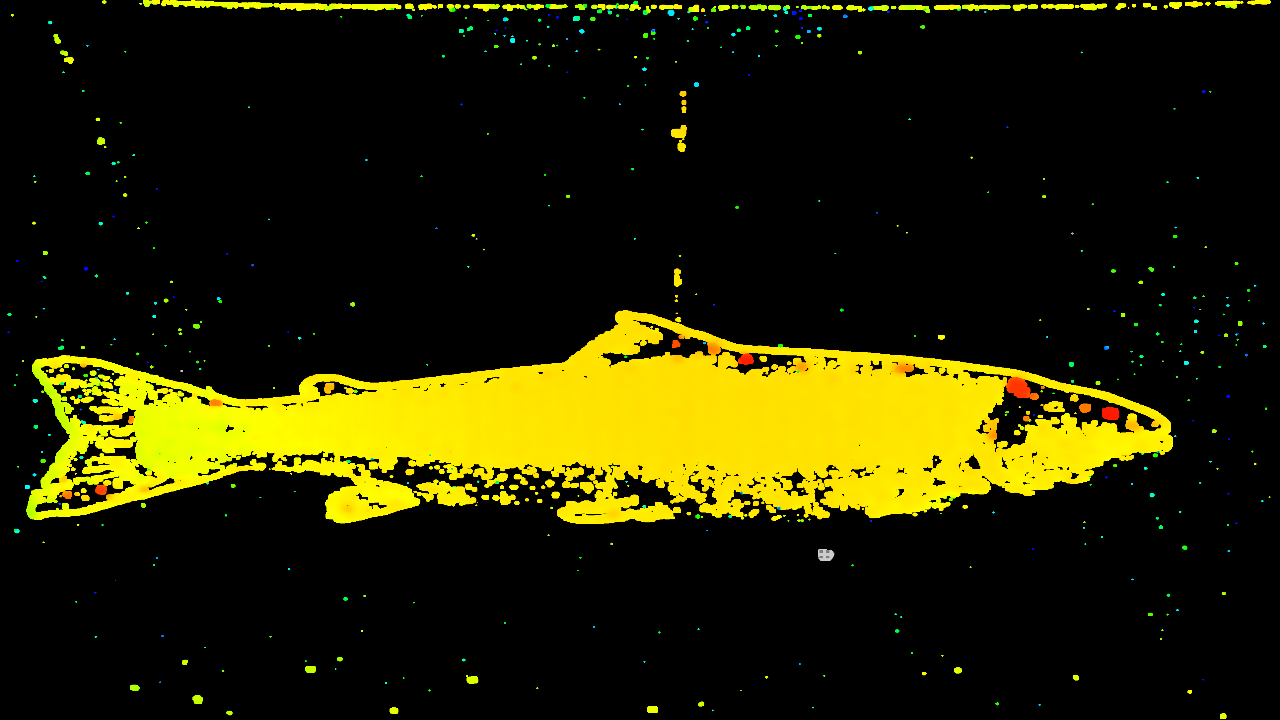
\includegraphics[width=\linewidth]{images/implementation/algorithm_test/original_82}
        \caption{Original depthmap image} 
        \label{fig:original_depthmap_82}
    \end{subfigure}\hspace*{\fill}
    \begin{subfigure}{0.48\textwidth}
        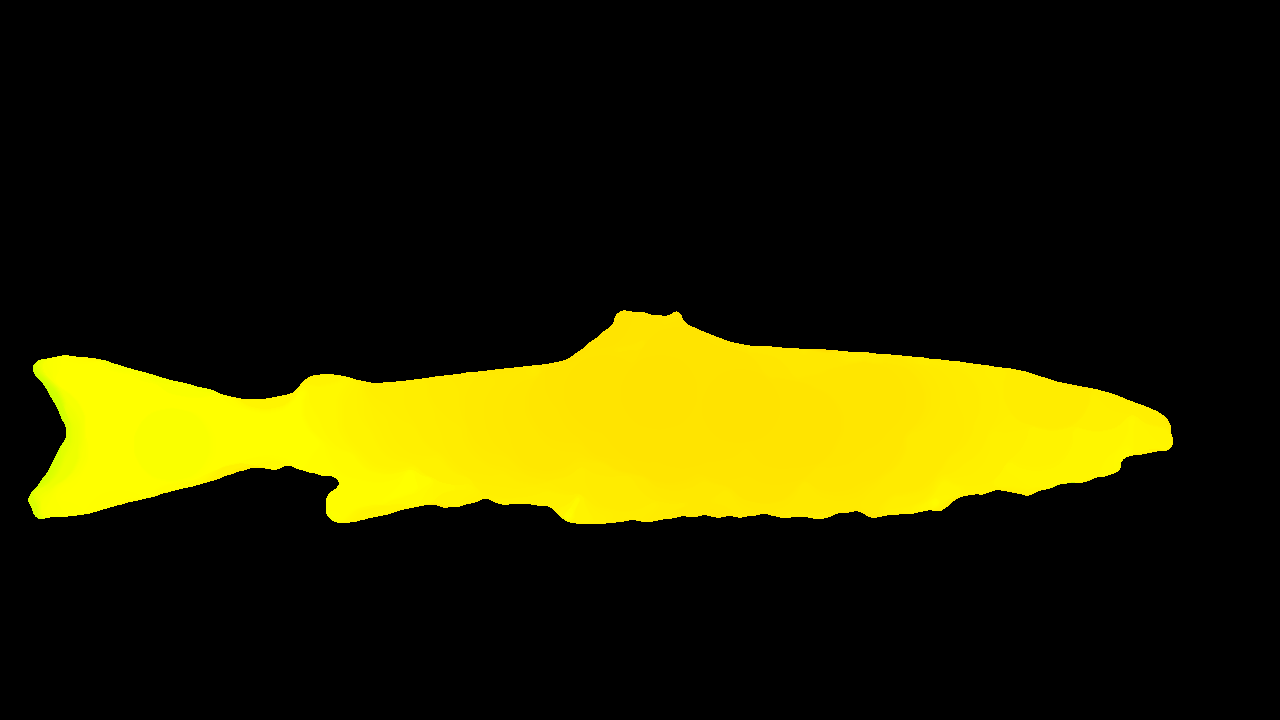
\includegraphics[width=\linewidth]{images/implementation/algorithm_test/median_filter_63}
        \caption{Result} 
        \label{fig:result_82}
    \end{subfigure}
    
    \medskip
    \begin{subfigure}{0.48\textwidth}
        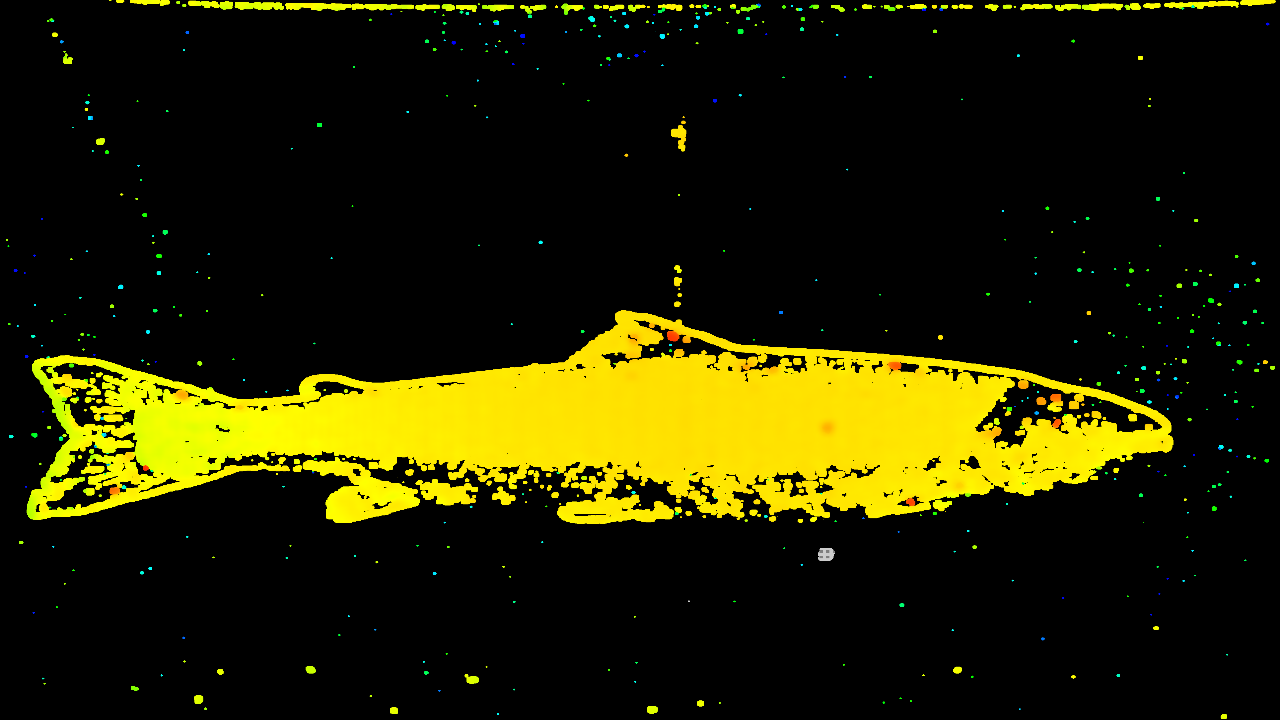
\includegraphics[width=\linewidth]{images/implementation/algorithm_test/original_87}
        \caption{Original depthmap image} 
        \label{fig:original_depthmap_87}
    \end{subfigure}\hspace*{\fill}
    \begin{subfigure}{0.48\textwidth}
        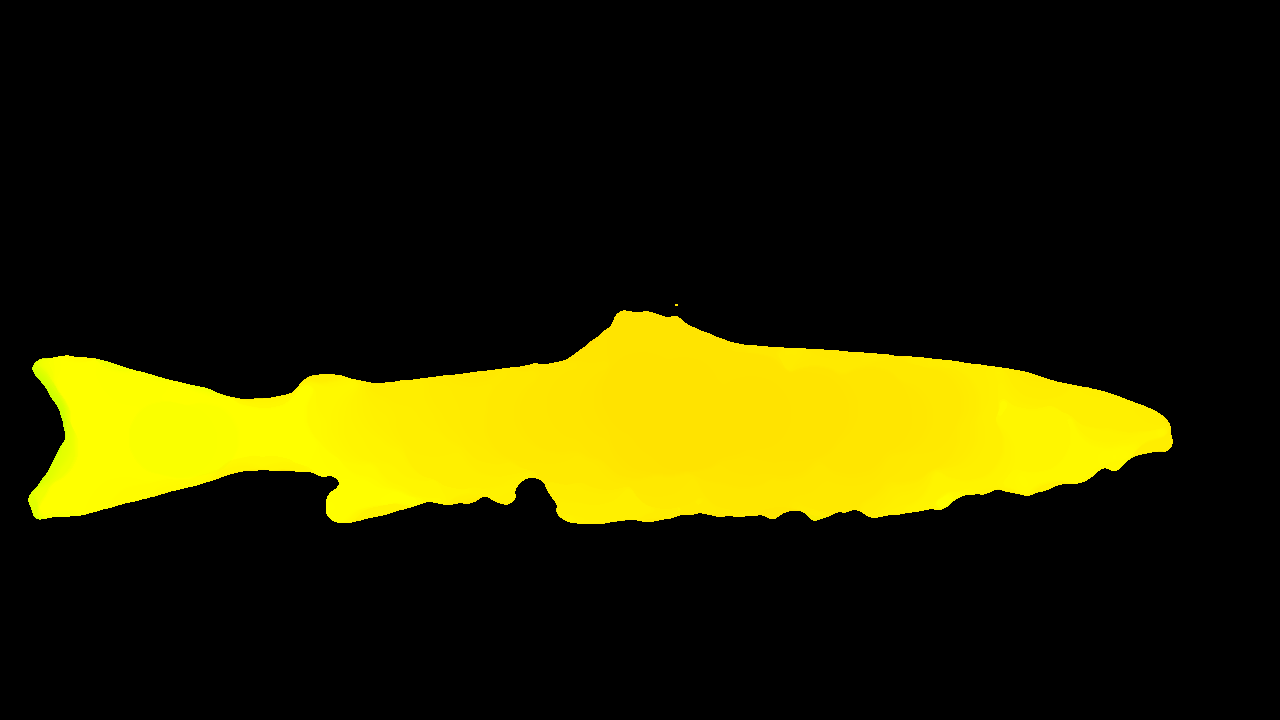
\includegraphics[width=\linewidth]{images/implementation/algorithm_test/median_filter_87}
        \caption{Result} 
        \label{fig:result_87}
    \end{subfigure}
    
    \caption{Algorithm test on different images} 
    \label{fig:algorithm_test}
\end{figure}

\newpage


%%%%%%%%%%%%%%%%%%%%%%%%%%%%%%%%%%%%%%%%%%%%%%%%%%%%%%%%%%%%%%%%%%%%%%


\subsection{Different Levels of Particle Noise} \label{section:noise}

To make the algorithm suitable for different conditions of water, noise was added to the depthmap.
The original plan was for the water to get blurry by it self since the dead salmons rotting process is very quick. The water, at the end of picture taking, looked very blurry and filled with particles, but it did not show much differences in the depthmap image. It's not known if it is mostly the water mediums properties that causes noise in the depthmap, and that particles are not enlarging this disorder significantly, or if enough particles within reason will disturb the depth measurements done by the Raytrix.

Since we could not get the naturally disturbances in the water to affect the depthmap directly, noise was added to the computed depthmap images.

The noise used is random sized color circles with random color placed randomly. The radius of each pixel is between 1 and 6 pixels. Noise was added from level 1 to 40, where level 1 starts with 20 particles, and each level adds 40 particles. That is, level 40 has 1,580 random particles in the image.

The algorithm has few problems up to level 20. Figure \ref{fig:noise_level_1}, and figure \ref{fig:noise_level_8} shows noise level 1 and 8, respectively, and shows few differences. After level 20, small parts of the fish starts missing (figure \ref{fig:noise_level_22}), and those holes get bigger and more concentrated up to level 40. Still, the algorithm can sometimes get decent results, an example is figure \ref{fig:noise_level_32}. Level 40 is almost covered with particles, and this would most likely never be a real issue, but the result is still not too bad.

If this technology is to be used in conditions containing more particles than from the test case used in this report, it is reasonable to believe that some more processing and tuning could give good results also then. The case would most likely be to fill in the missing parts even more, and perhaps calculate the largest contour from the totalfocus image instead of the depthmap. 





{\color{red} Put this in result???

It is seen from the noisy images that it has almost no effect on the result. This shows that the algorithm is robust and will work in most particle conditions as long as the light settings remains the same and the distance to the fish is within some boundaries. }


\begin{figure}[H]
    \centering
    \begin{subfigure}{0.5\textwidth}
        \centering
        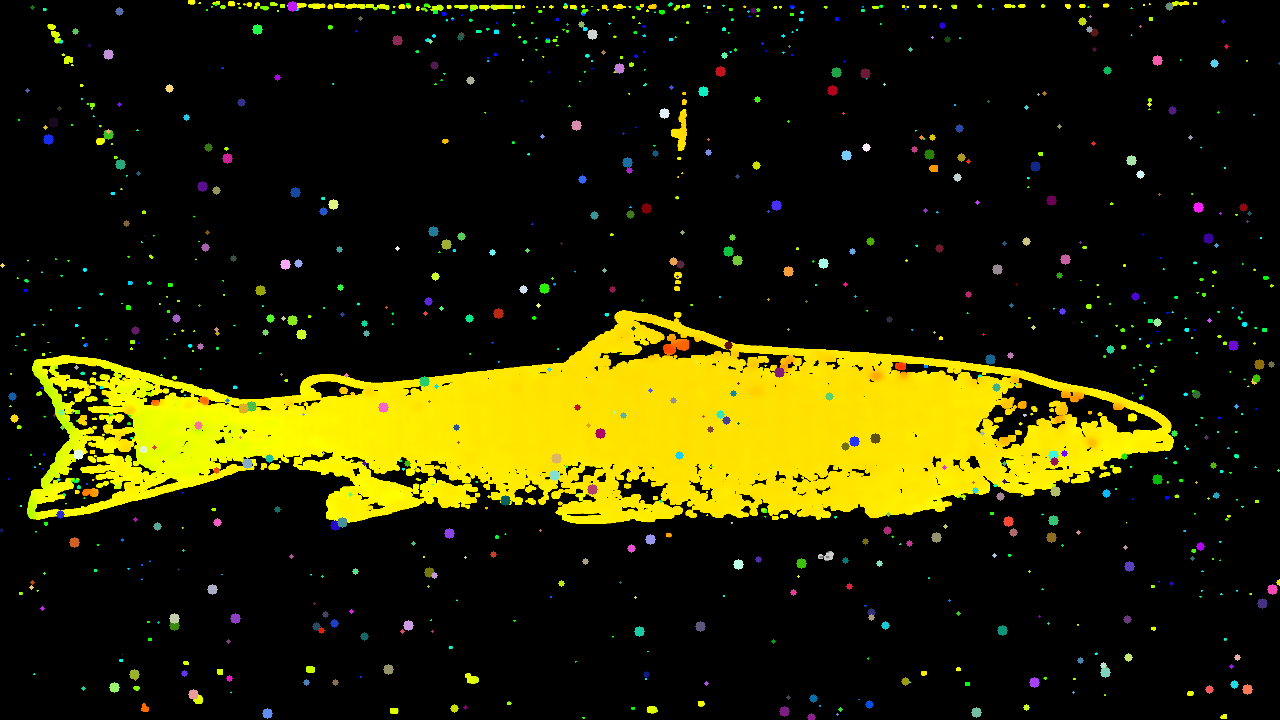
\includegraphics[width=.95\linewidth]{images/implementation/noise/noise63_1}
        \caption{Depthmap image with noise level 1} 
        \label{fig:image_noise_level_1}
    \end{subfigure}%
    \begin{subfigure}{0.5\textwidth}
        \centering
        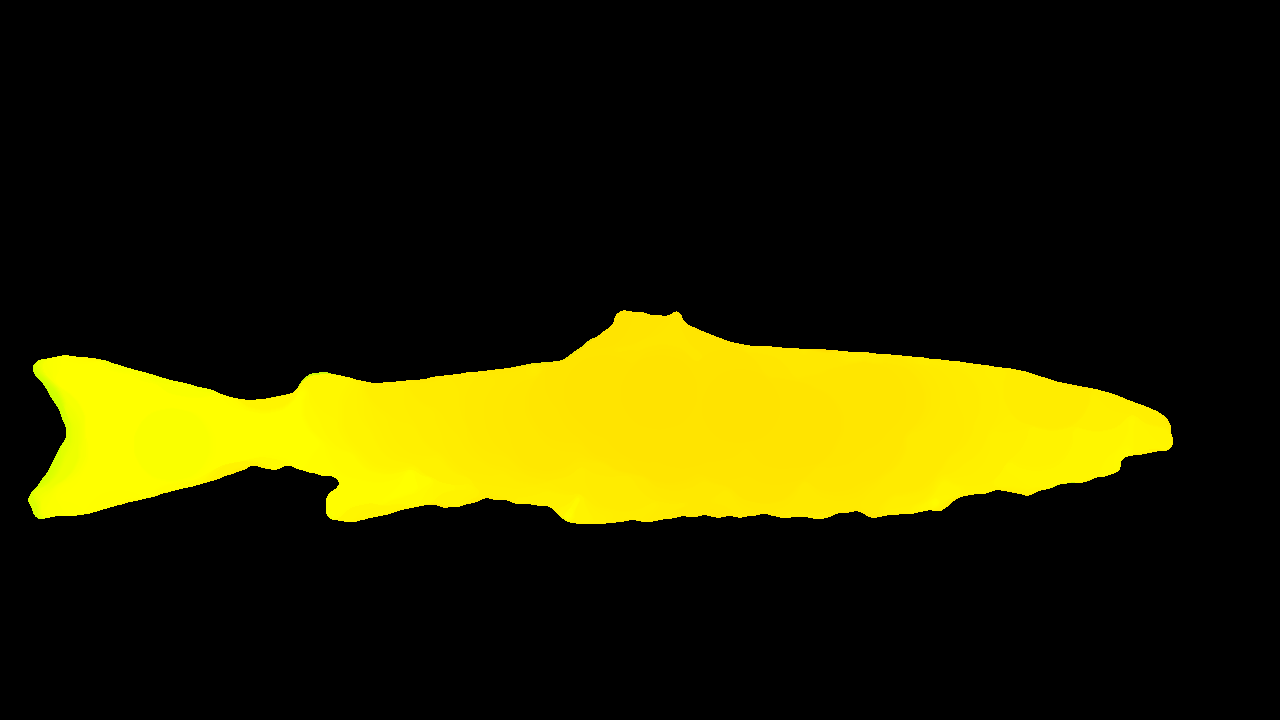
\includegraphics[width=.95\linewidth]{images/implementation/noise/filternoise63_1}
        \caption{Resulting depthmap} 
        \label{fig:filter_noise_level_1}
    \end{subfigure}
    \caption{Depthmap image and result for noise level 1}
    \label{fig:noise_level_1}
\end{figure}

\begin{figure}[H]
    \centering
    \begin{subfigure}{0.5\textwidth}
        \centering
        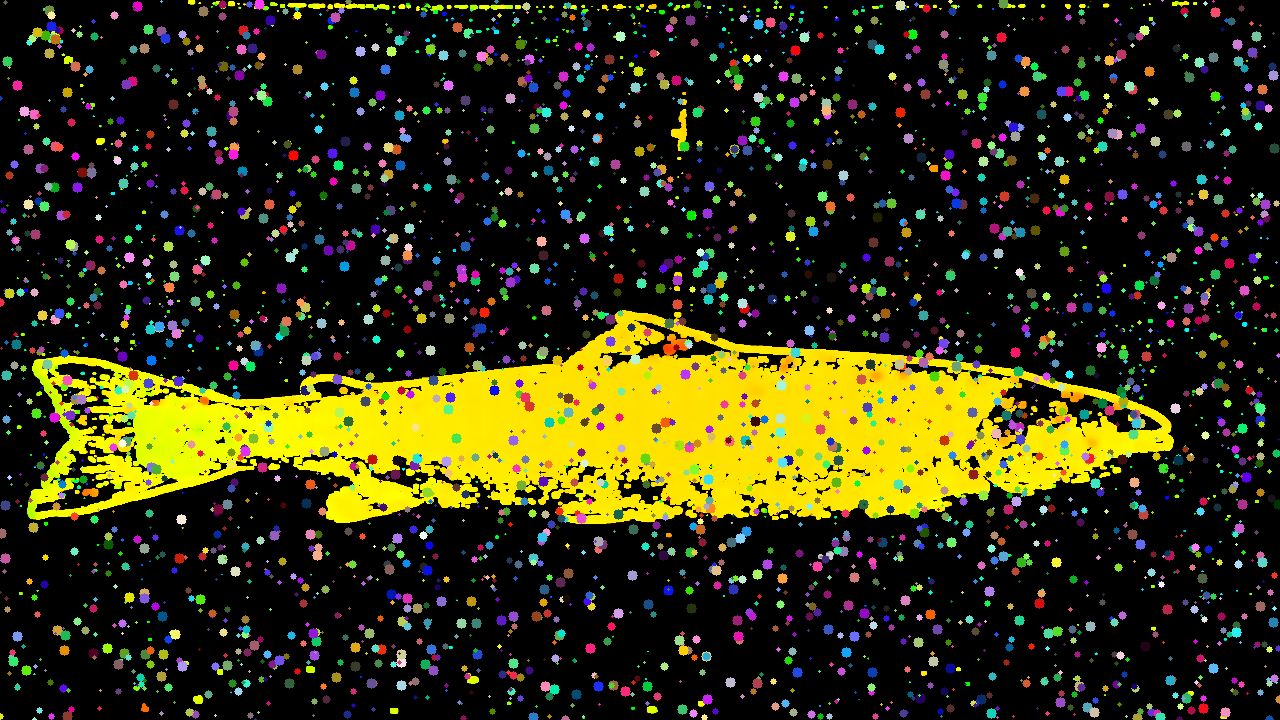
\includegraphics[width=.95\linewidth]{images/implementation/noise/noise63_8}
        \caption{Depthmap image with noise level 8} 
        \label{fig:image_noise_level_8}
    \end{subfigure}%
    \begin{subfigure}{0.5\textwidth}
        \centering
        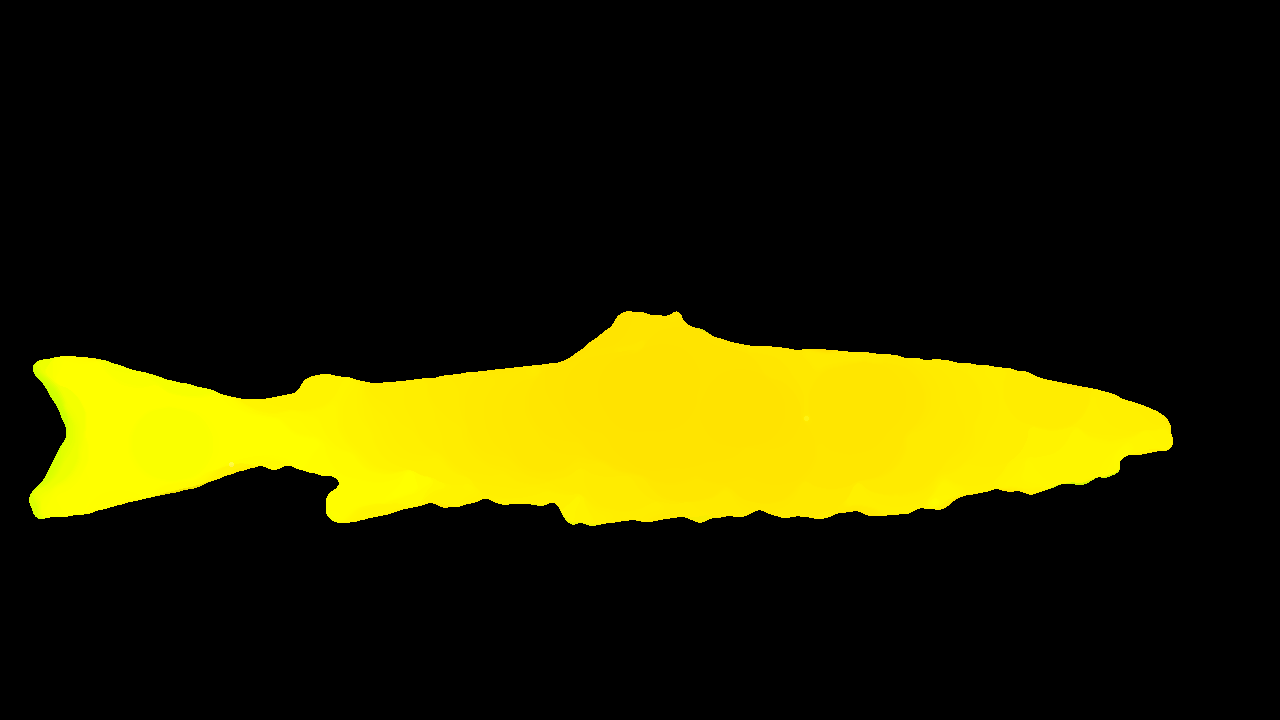
\includegraphics[width=.95\linewidth]{images/implementation/noise/filternoise63_8}
        \caption{Resulting depthmap} 
        \label{fig:filter_noise_level_8}
    \end{subfigure}
    \caption{Depthmap image and result for noise level 8}
    \label{fig:noise_level_8}
\end{figure}

\begin{figure}[H]
    \centering
    \begin{subfigure}{0.5\textwidth}
        \centering
        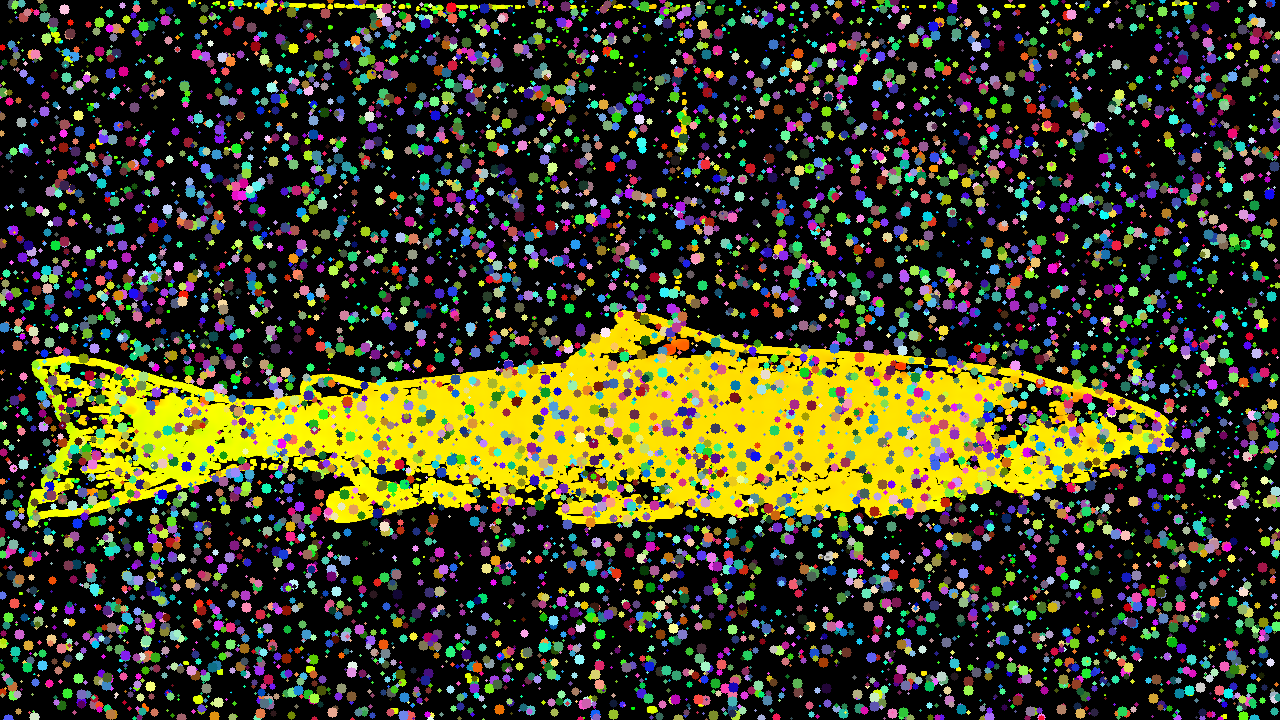
\includegraphics[width=.95\linewidth]{images/implementation/noise/noise63_22}
        \caption{Depthmap image with noise level 22} 
        \label{fig:image_noise_level_22}
    \end{subfigure}%
    \begin{subfigure}{0.5\textwidth}
        \centering
        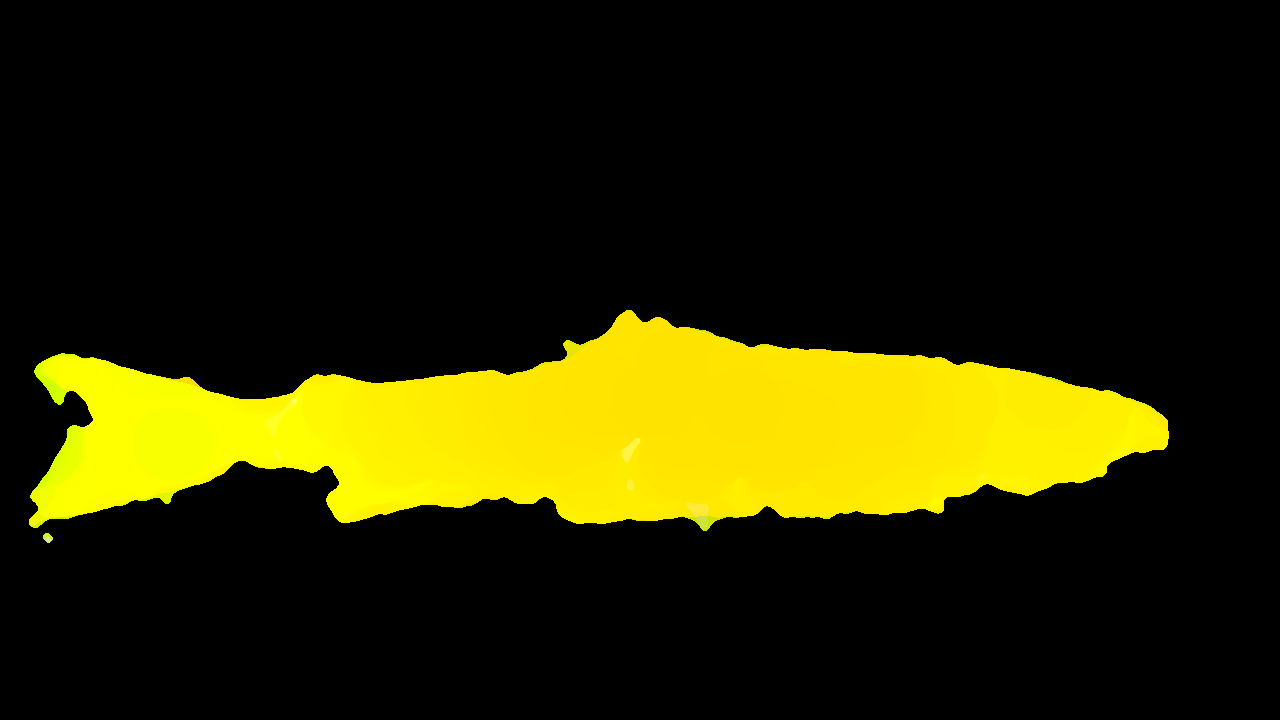
\includegraphics[width=.95\linewidth]{images/implementation/noise/filternoise63_22}
        \caption{Resulting depthmap} 
        \label{fig:filter_noise_level_22}
    \end{subfigure}
    \caption{Depthmap image and result for noise level 22}
    \label{fig:noise_level_22}
\end{figure}

\begin{figure}[H]
    \centering
    \begin{subfigure}{0.5\textwidth}
        \centering
        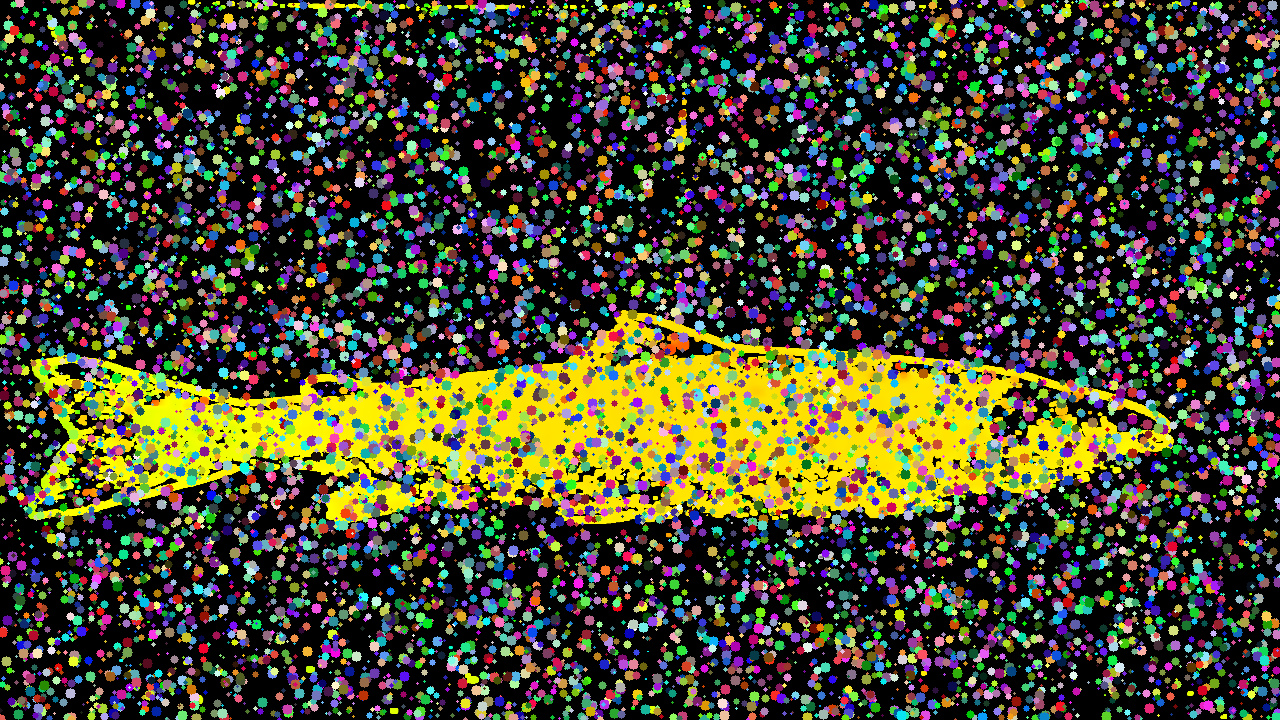
\includegraphics[width=.95\linewidth]{images/implementation/noise/noise63_32}
        \caption{Depthmap image with noise level 32} 
        \label{fig:image_noise_level_32}
    \end{subfigure}%
    \begin{subfigure}{0.5\textwidth}
        \centering
        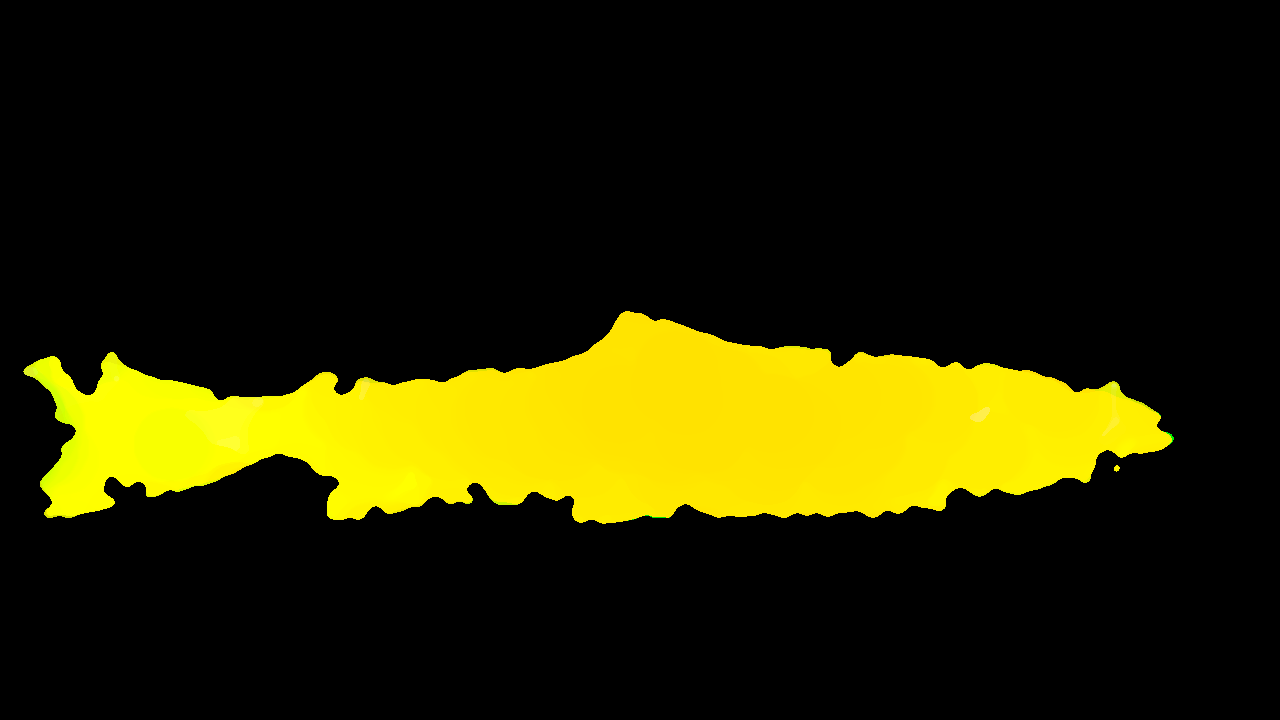
\includegraphics[width=.95\linewidth]{images/implementation/noise/filternoise63_32}
        \caption{Resulting depthmap} 
        \label{fig:filter_noise_level_32}
    \end{subfigure}
    \caption{Depthmap image and result for noise level 32}
    \label{fig:noise_level_32}
\end{figure}

\begin{figure}[H]
    \centering
    \begin{subfigure}{0.5\textwidth}
        \centering
        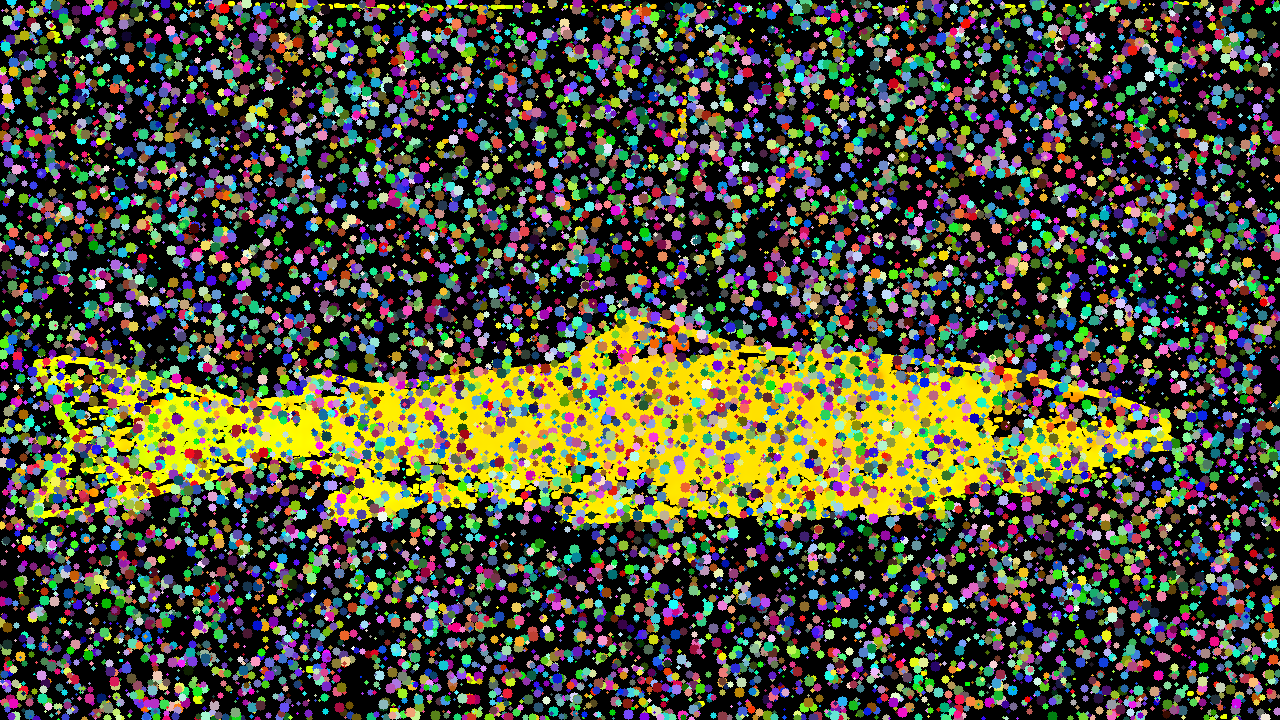
\includegraphics[width=.95\linewidth]{images/implementation/noise/noise63_40}
        \caption{Depthmap image with noise level 40} 
        \label{fig:image_noise_level_40}
    \end{subfigure}%
    \begin{subfigure}{0.5\textwidth}
        \centering
        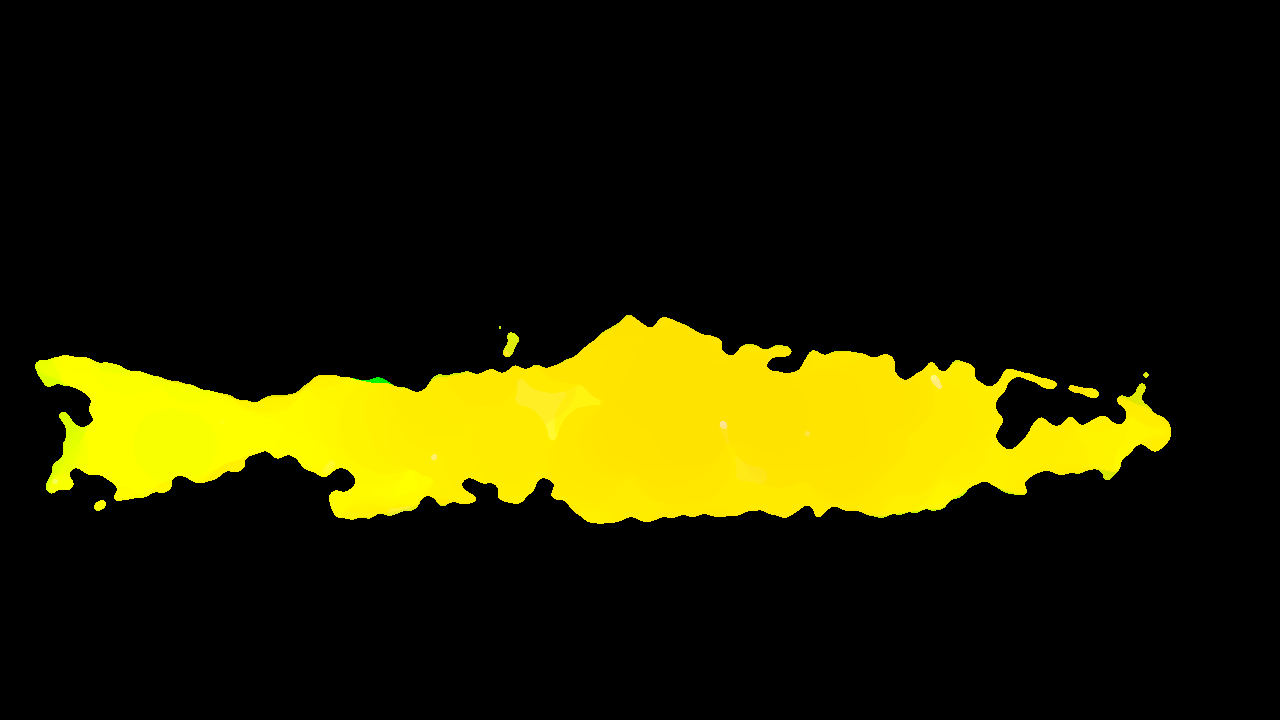
\includegraphics[width=.95\linewidth]{images/implementation/noise/filternoise63_40}
        \caption{Resulting depthmap} 
        \label{fig:filter_noise_level_40}
    \end{subfigure}
    \caption{Depthmap image and result for noise level 40}
    \label{fig:noise_level_40}
\end{figure}
